\chapter{预备知识}
\section{基础知识}
\subsection{函数的概念和特性}
\subsubsection{函数}
设$ x $与$ y $是两个变量, $ D $是一个给定的数集, 若对于每一个$ x\in D $, 按照一定的法则$ f $, 有一个唯一确定的$ y $与之对应, 则称$ y $为$ x $的函数, 记为$ y=f(x) $, 称$ x $为自变量, $ y $为因变量, $ D $为定义域.
\subsubsection{反函数}
设函数$ y=f(x) $的定义域为$ D $, 值域为$ R $, 若对于每一个$ y\in R $, 必存在唯一的$ x\in D $使得$ y=f(x) $成立, 则由此定义了一个新的函数$ x=\varphi(y) $, 称这个函数是$ y=f(x) $的反函数, 一般记作$ x=f^{-1}(y) $, 它的定义域为$ R $, 值域为$ D $. \par
\begin{tcolorbox}
\begin{enumerate}
\item 严格单调的函数一定有反函数(严格单调函数不一定是反函数, 如某些分段函数)
\item $ x=f^{-1}(y) $和$ y=f(x) $是同一个函数, 只有写成$ y=f^{-1}(x) $, 图像才关于$ y=x $对称
\end{enumerate}
\end{tcolorbox}
\subsubsection{复合函数}
函数$ u=g(x) $在$ x\in D $上有定义, 函数$ y=f(u) $在$ u\in D_{1} $上有定义, 且$ g(D)\subset D_{1} $, 则称$ y=f(g(x)) $为复合函数, 定义域为$ D $, $ u $为中间变量.
\subsubsection{函数的四种特性和重要结论}
\begin{enumerate}
\item 有界性\par
设$ f(x) $的定义域为$ D $, 数集$ I\subset D $. 若存在某个正数$ M $, 使得对于任一$ x\in I $, 有$ |f(x)|\le M $成立, 则称$ f(x) $在$ I $上有界. 如果这样的$ M $不存在, 则称$ f(x) $在$ I $上无上界.
\item 单调性\par
设$ f(x) $的定义域为$ D $, 区间$ I\subset D $, 如果对于区间上的任一两点$ x_{1},x_{2} $, 当$ x_{1}<x_{2} $的时候有$ f(x_{1})<f(x_{2}) $成立, 则称$ f(x) $在$ I $上单调增加. 反之如果$ f(x_{1})>f(x_{2}) $成立, 则称$ f(x) $在$ I $上单调减少.
\item 奇偶性\par
设$ f(x) $的定义域$ D $关于原点对称. 如果对于任一$ x\in D $, 恒有$ f(x)=f(-x) $, 则称$ f(x) $为偶函数. 如果对于任一$ x\in D $, 恒有$ f(x)=-f(-x) $, 则称$ f(x) $为奇函数. 偶函数的图像关于$ y $轴对称, 奇函数的图像关于原点对称.
\begin{tcolorbox}
\begin{enumerate}
\item 奇函数在$ 0 $点有定义则$ f(0)=0 $
\item 偶函数当$ f'(0) $存在时则$ f'(0)=0 $
\item 函数$ f(x) $和$ -f(x) $关于$ x $轴对称, 函数$ f(x) $和$ f(-x) $关于$ y $轴对称, 函数$ y(x) $和$ -y(-x) $关于原点对称
\item 函数$ f(x) $关于$ x=T $对称$ \Leftrightarrow f(x+T)=f(T-x) $
\end{enumerate}
\end{tcolorbox}
\item 周期性\par
设$ f(x) $的定义域为$ D $, 若存在一个正数$ T $, 使得对于任一$ x\in D $, 有$ x\pm T\in D $, 且$ f(x+T)=f(x) $. 则称$ f(x) $为周期函数, $ T $称为$ f(x) $的周期.
\item 重要结论
\begin{enumerate}
\item 函数和其导函数
\subitem 偶函数的导函数是奇函数
\subitem 奇函数的导函数是偶函数
\subitem 周期函数的周期和其导函数的周期相同
\item 函数和其原函数
\subitem 连续的奇函数的原函数是偶函数
\subitem 连续的偶函数的原函数只有一个是奇函数
\subitem 连续的周期函数和其原函数的周期相同
\item 若$ f(x) $在$ (a,b) $内可导且$ f'(x) $有界, 则$ f(x) $在$ (a,b) $内有界
\end{enumerate}
\end{enumerate}
\subsection{函数的图像}
\subsubsection{直角坐标系}
\begin{enumerate}
\item 常见图像
\begin{enumerate}
\item 基本初等函数与初等函数
\begin{enumerate}
\item 常数函数\par
$ y=C $, $ C $为常数, 图形为平行于$ x $轴的水平直线.
\item 幂函数\par
$ y=x^{\mu} $\ ($ \mu $是实数)
\begin{tcolorbox}
\begin{enumerate}
\item 见到$ \sqrt{u},\sqrt[3]{u} $, 用$ u $来研究最值
\item 见到$ |u| $时, 用$ u^{2} $来研究最值
\item 见到$ u_{1}u_{2}u_{3} $时, 用$ ln(u_{1}u_{2}u_{3})=lnu_{1}+lnu_{2}+lnu_{3} $来研究最值
\item 见到$ \frac{1}{u} $时, 用$ u $来研究最值
\end{enumerate}
\end{tcolorbox}
\item 指数函数
$ y=a^{x} $\ ($ a>0,a\neq 1 $)
\item 对数函数
$ y=log_{a}x $\ ($ a>0,a\neq 1 $)
\begin{tcolorbox}
常用公式: $ x=e^{lnx}\ (x>0), u^{v}=e^{lnu^{v}}=e^{vlnu}\ (u>0) $
\end{tcolorbox}
\item 三角函数
\begin{enumerate}
\item 正弦函数和余弦函数\par
正弦函数$ y=\sin x $, 余弦函数$ y=\cos x $.
\item 正切函数和余切函数\par
正切函数$ y=\tan x $, 余切函数$ y=\cot x $.\par

\begin{figure}[htp]
\centering
\begin{tikzpicture}[
>=stealth
]
\draw[->] (-1,0)--(4,0)node[right]{$ x $};
\draw[->] (0,-1)--(0,4)node[right]{$ y $};
\node at (-.2,-.2){$ 0 $};
\draw[] (1,0)node[below]{$ 1 $}--(1,.1);
\foreach \x in {1,2,3,...,6}{
\draw[] (0,\x*0.5)node[left]{$ \x $}--(.1,\x*0.5);
\node at (.2,.2){$ 0 $};
}
\end{tikzpicture}
\end{figure}
\begin{figure}[htp]
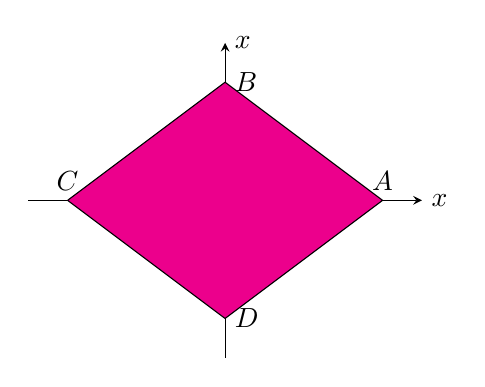
\begin{tikzpicture}[
>=stealth,
scale=.5,
]
\draw[->] (-5,0)to(5,0)node[right]{$ x $};
\draw[->] (0,-4)to(0,4)node[right]{$ x $};
\draw[fill=magenta] (-4,0)node[above]{$ C $}to(0,3)node[right]{$ B $}to(4,0)node[above]{$ A $}to(0,-3)node[right]{$ D $}to(-4,0);
\end{tikzpicture}
\end{figure}
\begin{figure}
\begin{tikzpicture}[
]
\draw[] content;
\end{tikzpicture}
\end{figure}
\end{enumerate}
\end{enumerate}
\end{enumerate}
\end{enumerate}






















